\documentclass[11pt]{article}
\usepackage[margin=0.85in]{geometry}
\usepackage{amsmath,graphicx,hyperref}
\setlength{\parindent}{0pt}\setlength{\parskip}{6pt}
\setlength{\emergencystretch}{3em}
\begin{document}
{\Large Saved cover inputs: occupancy and representation}\\
November 13, 2026. Unsigned native audit [pcc:unverified].

The two completed round5 records each have16 distinct image abscissas, but
only6 reference and8 cubic abscissas pass the nonzero-square filter. The cubic
count matches its saved field; the reference count was absent. Both target
abscissas are rational on their respective curves. These are different curves
and planted targets, not a general cubic-map density advantage.

\begin{center}
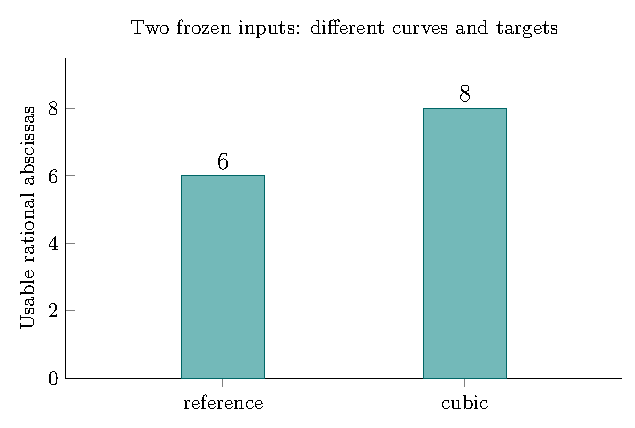
\includegraphics[width=0.87\linewidth]{base-counts.pdf}
\end{center}

\textbf{Exact check.} The frozen Rust validator \path{bf27909df} pins both
input digests, checks the31-bit prime and curve nonsingularity, primitive16th
root, coset distinctness, images and all32 point/residue calculations. Neither
case has a zero-$y$ abscissa. Full point records are retained. It does not replay
F4, its basis or planted solution, prove subgroup order, recover a scalar or
measure useful-relation yield. Statement \path{PCC-20261113-79248f} pins the
unsigned data artifact; PCC reports not\_covered.

\textbf{Original gate retained.} The reported W-only cubic cell remains C:
245930 versus167726 columns. Its same-seed retry alone completed after the
shared-pod kill. Quart/generic3 remain censored. The producer corrected the
late erroneous hard-stop text and preserved it. Different curve/target draws,
only one planted target per arm and mixed concurrency limit total-cost
interpretation. This audit does not change the frozen finite W gate.

\textbf{Encoding observation.} Frozen source \path{3466f3be9e} substitutes
cubic $N(u)$ directly into S3; raw input degrees12,8,8 versus4,4,4 for the
reference. The recorded last productive degree is7. Explicit image-coordinate
variables are a distinct standard representation to test.

\newpage
{\Large Graph correspondence and the proposed next test}

Introduce $x_i=N(u_i)$ and use ordinary S3 in the new image coordinates.
For this polynomial cover there are no denominator guards. The proposed m4
layout has22 variables/23 equations and maximum input degree4. These are
unimplemented-builder predictions. Added variables may outweigh any benefit;
lower input degree does not imply less work or a sub-exponential bound.

\textbf{Formal map.} \path{CoverGraph.lean}, frozen source \path{75e4b203e},
defines original solutions, lifted solutions and the actual lift/project maps
for arbitrary map $\phi$ and residual predicate. The theorems projectLift and
liftProject establish both inverse identities. This proves generic pointwise
solution correspondence, not an actual polynomial builder, degree bound or
solver complexity. It is standard graph substitution, with no novelty claim.

\begin{center}
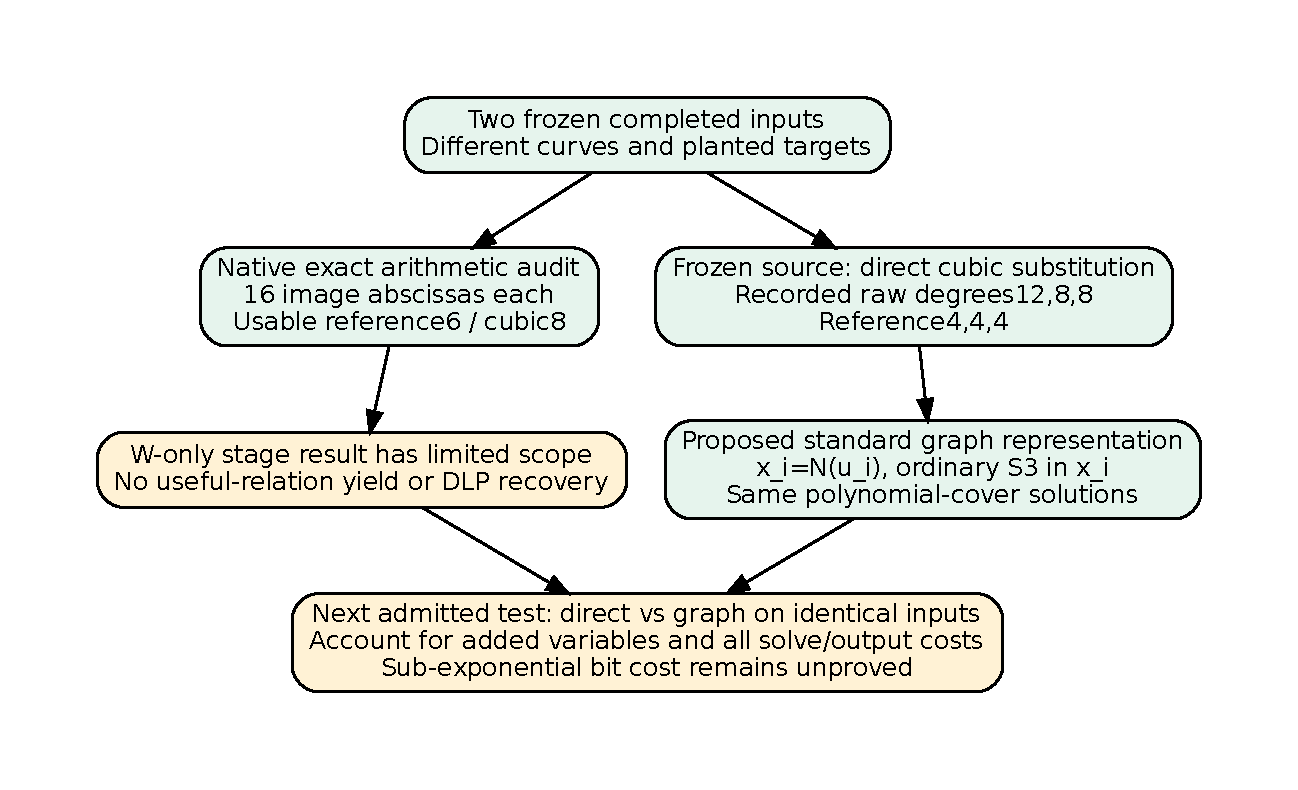
\includegraphics[width=0.97\linewidth,height=0.32\textheight,keepaspectratio]{encoding.pdf}
\end{center}

\textbf{Checks and failures.} Native16 tests pass after adding the omitted
pinned hex test dependency; failed test001 retained. Graph builds001/002 fail
on opaque subtype compilation/core-only Type* syntax;003 uses exposed aliases
and explicit universes, completes3 jobs and reports no axioms for either
identity. Source audit and fresh import-inclusive replay have attributable
receipts. The premature failed-source commit remains a failed stage.

\textbf{Next admitted experiment.} Compare direct and graph systems on exactly
the same literal curve, coset, map and target. Validate both projection
directions and known-answer witnesses, then count actual sparse work and all
solve/output costs. Measure positive and naturally negative cases separately.
Record usable base sizes and setup rejection costs; do not assume relation
yield from the observed6/8 pair. Preserve memory failures and isolate resources
for time comparisons. The draft protocol remains unexecuted.

\textbf{Sources and resources.} Original protocol and amendments, launch
scripts, saved rows, progress log and binary digest; frozen map, summation and
generator code; prior auxiliary-cover review. KB MCP/wrapper unavailable, bounded GitHub
fallback. Native correctness only: no new target, solver, timing/scaling run
or paid job. Live compute admission is unconfirmed. No benchmark, leaderboard
or ecdb result. A sub-exponential public-input finder and its bit cost remain
open. Editable source, data, DOT/SVG and exact receipts accompany this report.
\end{document}
